\documentclass[11pt]{beamer}
\usepackage{listings} % Include the listings-package
\usepackage[T1]{fontenc}
\usepackage[utf8]{inputenc}
\usepackage[english]{babel}
\usepackage{amsmath}
\usepackage{amssymb, amsfonts, latexsym, cancel}
\usepackage{float}
\usepackage{graphicx}
\usepackage{epstopdf}
\usepackage{subfigure}
\usepackage{hyperref}
%\usepackage{authblk}
\usepackage{blindtext}
\usepackage{booktabs} % Allows the use of \toprule, 
\usepackage{filecontents}
\usepackage{courier} %% Sets font for listing as Courier.
\usepackage{listings}

\usepackage{graphicx} %package to manage images
\graphicspath{ {./images/} }



%\usepackage{listings, xcolor}
\lstset{
tabsize = 2, %% set tab space width
showstringspaces = false, %% prevent space marking in strings, string is defined as the text that is generally printed directly to the console
numbers = left, %% display line numbers on the left
commentstyle = \color{green}, %% set comment color
keywordstyle = \color{blue}, %% set keyword color
stringstyle = \color{red}, %% set string color
rulecolor = \color{black}, %% set frame color to avoid being affected by text color
basicstyle = \small \ttfamily , %% set listing font and size
breaklines = true, %% enable line breaking
numberstyle = \tiny,
}
\usepackage{caption}
\DeclareCaptionFont{white}{\color{white}}
\DeclareCaptionFormat{listing}{\colorbox{gray}{\parbox{\textwidth}{#1#2#3}}}
\captionsetup[lstlisting]{format=listing,labelfont=white,textfont=white}
\definecolor{urlColor}{rgb}{0.06, 0.3, 0.57}
\definecolor{linkColor}{rgb}{0.57, 0.0, 0.04}
\definecolor{fileColor}{rgb}{0.0, 0.26, 0.26}
\hypersetup{
    colorlinks=true,
    linkcolor=linkColor,
    filecolor=fileColor,      
    urlcolor=urlColor,
}
\urlstyle{same}
\setbeamercovered{transparent}
%\usetheme{Boadilla}
%\usetheme{CambridgeUS}
%\usetheme{Berkeley}
%\usetheme{Warsaw}
\usetheme{Madrid}

\title[Presentación]{\bf\Huge Videojuegos }
\subtitle{Interaccion Humano Computador}

\author[]
{
	Grupo LOS AMIGUITOS\\ 
	Mariana Grethel Yucra Machaca \inst{1}\\
	Valery Byrne Macias \inst{1}\\
	Aldair Salcedo Chavez \inst{1}\\
	Victor Manuel Vilca Rojas  \inst{1}\\
	Deyner Junior Patiño Mendoza \inst{1}\\
}
\institute[UNSA]
{
\inst{1}% 
System Engineering School\\
System Engineering and Informatic Department\\
Production and Services Faculty\\
San Agustin National University of Arequipa
}

\date[2020-09-14]{\scriptsize{2020-09-14}}
%\logo{\includegraphics[width=3.0cm]{img/logo_unsa.jpg}}
%\titlegraphic{\includegraphics[width=1.0cm]{img/logo_unsa.jpg}}

\begin{document}

\begin{frame}
\titlepage
\end{frame}

\begin{frame}
\frametitle{Content}
\tableofcontents
\end{frame}


\section{Rivit}
\begin{frame}
\frametitle{Rivit}
\begin{itemize}
\item Propósito: Ayudar a pacientes con problemas cardíacos.
\item Colección de minijuegos que ayudan al desarrollo de habilidades cognitivas.
\item Tres grupos evaluados: 30 > p; 60< p ;  30<p<60
\item Dificultades en comprensión.

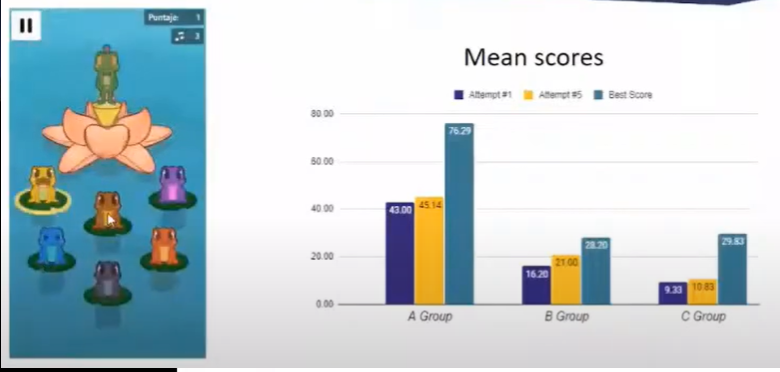
\includegraphics[width=5cm, height=2cm]{images/rivit2.png}
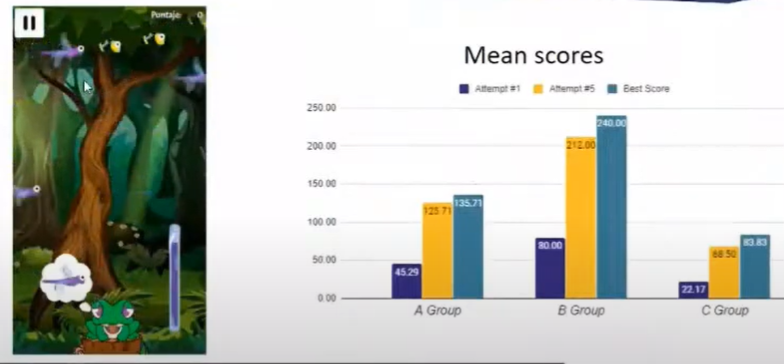
\includegraphics[width=5cm, height=2cm]{images/rivit3.png}
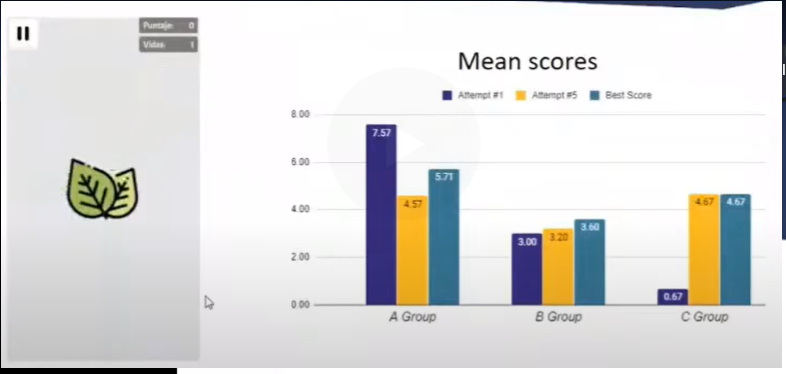
\includegraphics[width=5cm, height=2cm]{images/rivit4.png}
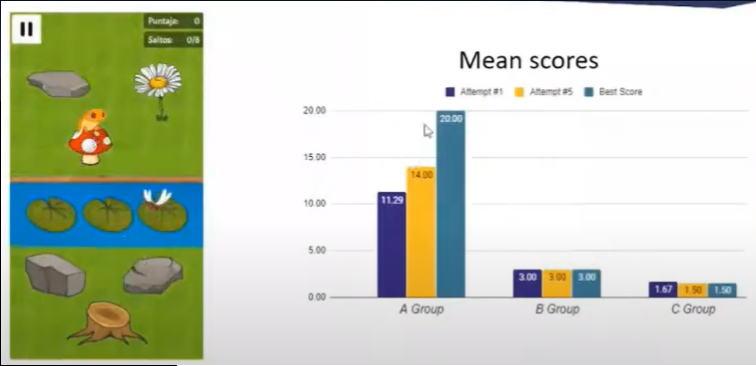
\includegraphics[width=5cm, height=2cm]{images/rivit5.png}

\end{itemize}
\end{frame}


\section{Tales of Etrya}
\begin{frame}
\frametitle{Tales of Etrya}
\begin{itemize}

\item Tales of Etrya es un videojuego que tiene como objetivo enseñar Inglés


\item Diseño colaborativo
\item Es útil para los profesores
\item  Herramienta de motivación 
\item Motivación a largo plazo
\item Genera interacción social , con otros estudiantes

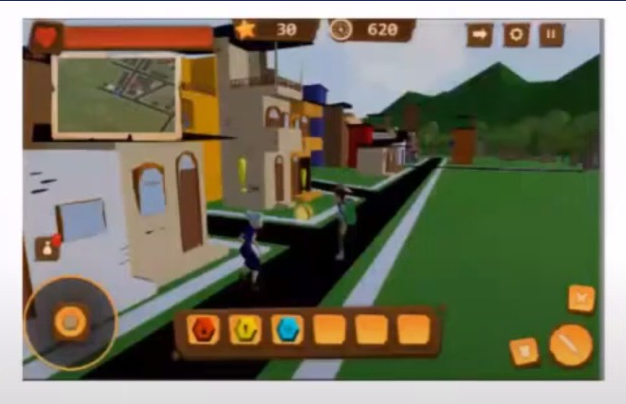
\includegraphics[width=6cm, height=5cm]{images/toe1.png}

\end{itemize}
\end{frame}

\section{Ninipolis}
\begin{frame}
\frametitle{Ninipolis}
\begin{itemize}
\item El juego digital Ninipolis simula realidades que experimentan los jovenes en el Perú.
\item Impulsado por la plataforma de activismo Actua.pe 
\item Se basa en los estudios de de Ana Paula Franco “Ser joven el Perú: educación y trabajo” y en “Jóvenes y desigualdad en un país cuesta arriba“de OXFAM en Perú.
\item Objetivo: Ponerte en lugar de los demás  jóvenes peruanos.
\item \href {https://youtu.be/hQPjfMj0rSk}{https://youtu.be/hQPjfMj0rSk}

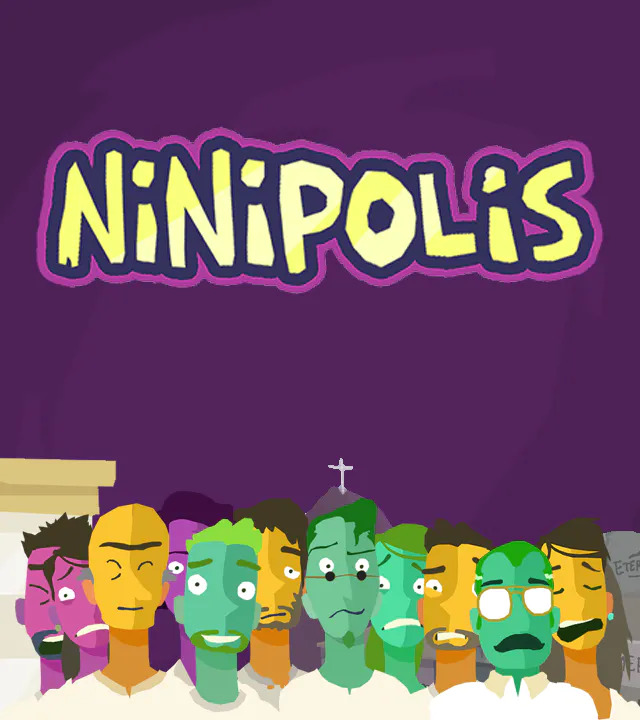
\includegraphics[width=4cm, height=4cm]{images/ninipolis1.png}

\end{itemize}
\end{frame}


\section{Conclusiones}
\begin{frame}
\frametitle{Conclusiones}
\begin{itemize}
\item De los diferentes trabajos que encontramos, podemos encontrar una idea en común, que es, tomar los videojuegos como herramientas beneficiosas para las personas. Estos beneficios pueden ser en cuanto a su salud, conocimiento, entretenimiento. Y no solo el hecho de jugarlos, el desarrollo de un videojuego es un proyecto que te permite poner en práctica las habilidades de los desarrolladores.



\end{itemize}
\end{frame}

\section{Referencias}
%References frame
\begin{frame}
\frametitle{References}
\begin{itemize}
\item \href{https://www.youtube.com/watch?v=mis-dKDgZJI&t=6357s}{https://www.youtube.com/watch?v=mis-dKDgZJI&t=6357s}
\item \href {https://www.youtube.com/watch?v=9pvekDuFxOw&t=1672s}{https://www.youtube.com/watch?v=9pvekDuFxOw&t=1672s}

\item \href {http://ninipolis.actua.pe/}{http://ninipolis.actua.pe/}



\end{itemize}
\end{frame}

\end{document}
